\section{Encoderinterfaces}

Naast dat er verschillende soorten motoren gebruikt worden bij Voortman worden er ook verschillende soorten encoders gebruikt in deze motoren die ook moeten communiceren met de motordrive van de motor. Het is daarom belangrijk om te begrijpen welke encoder soorten er allemaal zijn en welke gebruikt worden bij Voortman.

\subsection{Verschillende encoders}

In tabel \ref{tab:GebruikteEncoders} is te zien welke soorten encoders Voortman heeft in de motoren die zij gebruiken. Al deze encoders worden dankzij de option encoder kaart allemaal ondersteunt.

\begin{table}[H]
	\caption{Gebruikte encoders}
	\label{tab:GebruikteEncoders}
	\centering
	\begin{tabular}{|p{0.4\linewidth}|p{0.4\linewidth}|}
		\hline
		\textbf{Motor} & \textbf{Encoder} \\
		\hline
		\textbf{MAD100D-0250-SA-C0-AK0-35-N3} & Optical encoder, single-turn EnDat2.1, with 2048 increments \\
		\textbf{MAD130C-0150-SA-S2-AP0-05-N1} & Optical encoder, single-turn EnDat2.1, with 2048 increments \\
		\textbf{HQL100X} & Incremental TTL 5V Rotary Analog RESO 4096 sig./turn \\
		\textbf{MSK101D-0450-NN-M1-AP0-NNNN} & Hiperface single turn 128 increments \\
		\textbf{MS2N10-D0BNN-AMVK0-NNNNN-NN} & Hiperface multiturn 4096 revolutions absolute BASIC 16 signals periods \\
		\hline
	\end{tabular}
\end{table}

\newpage

\subsubsection{Incremental vs. absolute encoders}

Een absolute encoder kan meteen de exacte positie vertellen van de as zelfs als de stroom net is ingeschakeld en wanneer de encoder multi-turn is kan de encoder zelfs vertellen hoeveel rotaties de encoder gemaakt heeft. Een incrementele encoder kan alleen een verschil doorgeven in positie en moet bij inschakelen eerst langs zijn referentie positie gaan voordat de incrementele encoder pas de echte positie weet van de as. \cite{web:EncoderDifference}

\subsubsection{Resolver vs. Digitale encoders}

Een resolver is een analoge sensor die werkt met wisselstroom. De resolver gebruikt een inductieve koppeling om de hoekpositie te meten. Het bestaat uit een rotor en stator met wikkelingen erin. Wanneer de rotor draait induceert het spanningen in de statorwikkelingen deze kunnen weer worden omgerekend naar de hoekpositie van de as. De resolver wordt vooral gebruikt in robuuste omgevingen zoals de luchtvaart en militaire toepassingen.

\vspace{0.5cm}

De digital encoder is een digitale sensor die werkt op basis van optische, magnetische of capacitieve principes. Optische encoders hebben een schijf met patronen erin en een optische sensor die licht detecteert waarmee de encoder de positie van de as mee kan bepalen. Magnetische sensoren maken gebruik van een magneet en een Hall-sensor om de rotatie te meten. \cite{web:EncodervsResolver}

\begin{table}[H]
	\caption{Resolver vs. digital encoder}
	\label{tab:ResolvervsDigital}
	\centering
	\begin{tabular}{|p{0.4\linewidth}|p{0.4\linewidth}|}
		\hline
		\textbf{Resolver} & \textbf{Digitale Encoder} \\
		\hline
		Analoge spanning die wordt verwerkt in een digitale positie. & Directe digitale output zoals incrementele pulsen (A/B/C) of een absolute positie zoals \gls{SSI}, BiSS, EnDat, etc. \\
		Lagere resolutie en nauwkeurigheid dan de meeste digital encoders. & Hoge resolutie en nauwkeurigheid. \\
		Zeer betrouwbaar bij extreme omgevingen zoals stof, vuil, trillingen en temperatuurverschillen. & Minder robuust. \\
		\hline
	\end{tabular}
\end{table}

\newpage

\subsection{AX5140 encoder configuratie}

Bij de \gls{AX5140} is er de optie om tot twee encoders tegelijkertijd te configureren en dit kan op een aantal verschillende kanalen. Echter is niet elk kanaal geschikt voor elk type encoder zo kan het standaard kanaal X11 alleen Resolvers en incrementele encoders uitlezen. Omdat Voortman ook absolute encoders gebruikt in hun servo motoren is er een extra optie kaart geïnstalleerd in de drive dit is de \gls{AX5701} die ervoor zorgt dat ook absolute encoders aangesloten kunnen worden op de drive echter kan deze optie kaart geen incrementele encoders uitlezen het is daarom onvermijdelijk dat de operator het input kanaal van de encoder moet gaan verwisselen bij bepaalde type motoren op de testkast. De parameters van de encoder zelf kunnen gemakkelijk worden uitgelezen door het programma en worden ingeladen in de drive wanneer de gebruiker dit wil.

\vspace{0.5cm}

Daarnaast moet er ook een voeding gekozen worden voor de encoder en een wachttijd voordat de encoder pas wordt gebruikt dit is omdat soms de lichtbron even moet opwarmen in de encoder, geheugenherstel, communicatieprotocol initialisatie of een zelfkalibratie. Deze opstart tijden zijn vaak erg kort:

\begin{enumerate}
	\item Incrementele encoders vaak <1ms.
	\item Absolute encoders (\gls{SSI}, BiSS, EnDat) meestal 50-500ms.
	\item Optische of magnetische encoders meestal tot 100ms.
\end{enumerate}

Maar deze tijden kunnen sterk variëren en soms tot wel een paar seconden zijn afhankelijk van of de encoders bijvoorbeeld \gls{EEPROM} of \gls{FRAM} hebben. Tot slot moet er worden gekozen of de encoder lineair is of roterend wat in dit geval altijd roterend zal zijn.

\begin{figure}[H]
	\centering
	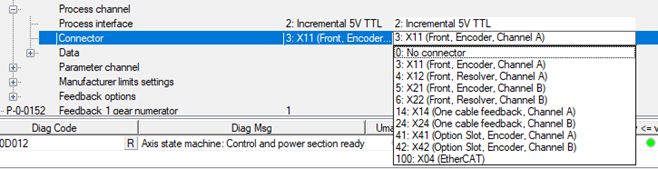
\includegraphics[width=350pt]{EncInputChannels}
	\label{fig:EncoderInputChannel}
	\caption{Encoder input channels}
\end{figure}

\begin{figure}[H]
	\centering
	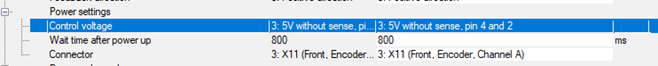
\includegraphics[width=350pt]{ControlVoltage}
	\label{fig:ControlVoltage}
	\caption{Encoder control voltage}
\end{figure}


